\capitulo{3}{Conceptos teóricos}
En esta sección vamos a centrarnos en explicar todos los conceptos necesarios para poder entender los pasos de los procesos realizados en la aplicación y saber en que se sustentan.

\begin{itemize}
\item Espacios de color: Las imágenes no son mas que matrices de números que expresan, valores o ponderaciones, distintos para representar los colores. La suma de todas ellas transmitido a través de un medio de reprodución, pantalla o similar, nos muestran las imágenes.
Cada espacio de color tiene unas propiedades y unas ventajas. Para obtener las característica que buscamos, con mayor o menor dificultad, por eso es necesario explicar los distintos espacios de colores.

\item Preprocesados:
Estos se compondrán de una serie de pasos previos a la obtención de los segmentos correspondientes a las estrías.
	\begin{itemize}
		\item La reducción de grosor: Es un paso clave en el procesado porque gracias a esto obtenemos los resultados que más se ajustan a la realidad.
No es complejo pero si que es muy útil, y sin este paso no serviría para nada nuestro procesado (su función es eliminar el ruido).
		\item Bordes: Al final, las estrías que detectamos no son más que bordes dentro de la imagen, y todo lo usado es para su detección, por lo que es necesaria su explicación. Como dato curioso, para la resolución de nuestro problema, lo que hemos hecho es reducirlo a un problema de detección de bordes.
	\end{itemize}

\item Análisis: 
Una vez que tengamos la máscara sobre la que detectar las características que estamos buscando, (este proceso tampoco sera directo) tendremos que dar  una serie de pasos para obtener nuestro objetivo.
	\begin{itemize}
	\item Transformada de Hough: Es un procedimiento matemático para buscar segmentos dentro de las imágenes binarizadas, dado que es complejo, es necesario explicar por que funciona y en qué consiste.

	\item Grafos: Gracias a la teoría de grafos podemos procesar muchos segmentos similares en uno solo, de forma sencilla y eficiente, por lo que precisa explicación.
	\end{itemize}

\end{itemize}



\section{Espacios de color }
El color que percibimos en los objetos que nos rodean depende de la radiación reflejada en ellos. Según los estudios, nosotros como humanos tenemos un rango <<de luz visible>> y ese rango son en verdad tres frecuencias diferentes, dentro del rango 769THz a 384THz~\cite{Manual:HAE}.
Así, la imagen que percibimos es la unión de las tres frecuencias diferentes, y para poder simular este hecho las máquinas simulan esta capacidad innata de los humanos creando los espacios de color que son modelos matemáticos para representar en una maquina lo que se observa en la figura \ref{fig:3.1}.

\begin{figure}[h]
\centering
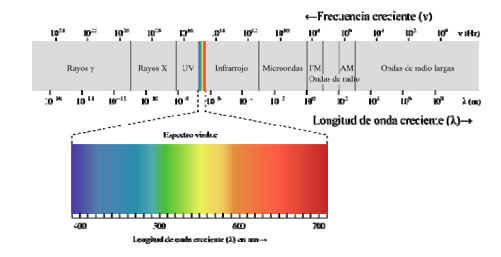
\includegraphics[width=.9\textwidth]{EspacioDeColor}
\caption{Frecuencias de luz visible \cite{Manual:HAE}}
\label{fig:3.1}
\end{figure}

\subsection{RGB}
El modelo RGB es usado por todos los sistemas digitales para la representación y captura de imágenes.

Se divide en tres canales, como se muestra en la figura \ref{fig:3.2}.

\begin{itemize}
	\item R: canal del rojo (RED) contiene la intensidad de rojo de cada pixel
	\item G: canal del verde (GREEN) contiene la intensidad de verde de cada pixel
	\item B: canal del azul (BLUE) contiene la intensidad de azul de cada pixel
\end{itemize}

\begin{figure}[h]
\centering
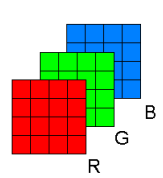
\includegraphics[width=.3\textwidth]{RGB_Canales}
\caption{Los tres canales del espacio RGB~\cite{Manual:HAE}}
\label{fig:3.2}
\end{figure}
La combinación de estos colores crea todas la gama de colores representable.
El valor de la intensidad de cada canal depende de la codificación usada para su representación (Ocho bits dan dieciséis millones de colores) como se muestra en la figura  \ref{fig:3.3}.

\begin{figure}[h]
\centering
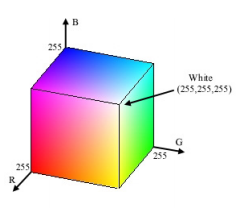
\includegraphics[width=.3\textwidth]{RGB}
\caption{Representación del modelo RGB~\cite{Manual:HAE}}
\label{fig:3.3}
\end{figure}

\subsection{HSV}
El modelo HSV \cite{modelo:hsv} esta orientado a la descripción de los colores en términos mas prácticos para el ser humano que el RGB, los canales significan algo más que la cantidad de cada color, por lo que es mas práctico para el ser humano. (Lo que se observa en la figura \ref{fig:3.4}).
 
\begin{itemize}
	\item H: (Matiz) que representa el tono o color.
	\item S: (Saturación) representa el nivel de saturación de un color.
	\item V: (Brillo) representa la intensidad lumínica.
\end{itemize}

\begin{figure}[h]
\centering
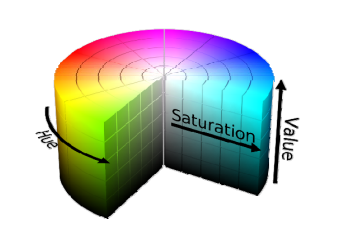
\includegraphics[width=.35\textwidth]{HSV}
\caption{Representación del modelo HSV~\cite{Manual:HAE}}
\label{fig:3.4}
\end{figure}

Una ventaja con otros espacios de color parecidos es que este permite representar todas las combinaciones del espacio RGB.
Pero su característica principal es que el canal de saturación, (representa la viveza de un color) y nos permitirá diferenciar las estrías del resto. Al seleccionar el color de las estrías pintadas, entre grises, que tendrán saturación muy baja, y el color pintado sobre éstas.

\subsection{CIELAB}
El modelo lab \cite{wiki:lab},mas conocido como CIELAB, es otra forma de representar los colores. Este en concreto, se basa en como representa los colores el ojo humano, la diferencia entre LAB y CIELAB, es que CIELAB utiliza raíces cúbicas, mientras que LAB usa raíces cuadradas.

El modelo lo podemos ver en la siguiente figura  \ref{fig:3.8}.

\begin{figure}[h]
\centering
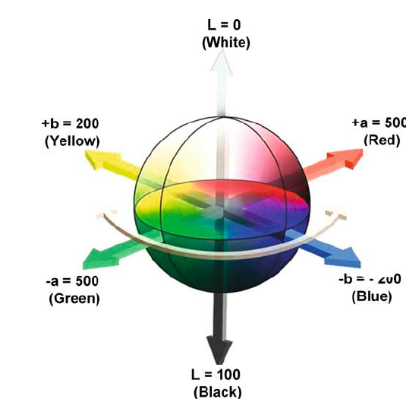
\includegraphics[width=.35\textwidth]{CieLAB}
\caption{Representación del modelo CIELAB~\cite{cie:LAB}}
\label{fig:3.8}
\end{figure}


Componentes del modelo:
\begin{itemize}
	\item L: Luminosidad de negro a blanco.
	\item A: Desde el color rojo al verde.
	\item B: Es la gradiente del color azul.
\end{itemize}

Ventajas:
\begin{itemize}
\item Corregir colores: Es más rápido hacer una corrección del color que en otros espacios de color.
\item Más cantidad de colores: Con esta representación del color conseguimos representar mayor número de colores, incluso colores imaginarios \footnote{Estos son colores que no es capaz de detectar el ojo humano, principalmente se usa para manipulación de imágenes.}.
\item La pérdida es mínima al cambiar a otro espacio de color.
\end{itemize}

El uso de este espacio de color viene dado por la necesidad de calcular la distancia a otros colores, que en este caso la diferencia. Caracteriza mejor que los demás espacios y por esto vamos a usar este espacio.
\section{Transformada de Hough }

Uno de los puntos relevantes del proyecto es la detección de las líneas pintadas o detectadas por el algoritmo (modo automático) y para ello vamos a usar una técnica que sirve para detectar formas, expresadas de forma matemática, dentro de imágenes.

Esta técnica fue inventada por Richard Duda y Peter Hart, en 1972 pero diez años antes, Paul Hough propuso y patentó \cite{pat:patHough} la idea inicial de detectar líneas en la imagen. Más tarde se generalizó para detectar cualquier figura.

\subsection{Teoría}

Normalmente, para detectar figuras sencillas en una imagen primero hay que usar algún algoritmo de detección de bordes o una binarización de la imagen, quedándonos con la región de interés apropiada (los píxeles que forman las rectas) pero normalmente faltan píxeles por el ruido en la imagen.

Para ello el método de Hough propone solucionar el problema detectando grupos de puntos que forman los bordes de la misma figura y así conseguir unirlos creando la recta real a la que pertenecen. Como podemos ver en el siguiente pseudocódigo 
\ref{alg:Hough}.

\label{alg:Hough}
%Hough
\begin{algorithm*}
\caption{Pseudocódigo de la transformada}
\DontPrintSemicolon
\KwIn{Imagen}
\KwOut{(list) de segmentos encontrados }

%$ S = \varnothing $

\ForEach {punto en la imagen}{
		\If {punto \textbf{(x,y)} esta en un borde:}{
			\ForEach {angulo en ángulos $\Theta$ }{
				Calcular $\rho$  para el punto (x,y) con angulo $\Theta$ \;
				Incrementar la posición ($\rho$ , $\Theta$ ) en el acumulador\;
			}
		}
}
Buscar las posiciones con mayores valores en el acumulador\;	

\Return {$rectas$ Las rectas cuyos valores son los mayores en el acumulador}
\end{algorithm*}

\subsection{Limitaciones}
Para que este proceso sea exitoso, los bordes del objeto deben ser detectados correctamente con un buen pre-procesado de la imagen y aparecer claramente las nubes de puntos que forman las rectas.
Como se muestra en la figura \ref{fig:3.5}.

\begin{figure}[h]
\centering
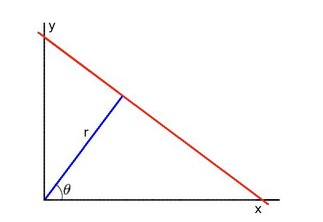
\includegraphics[width=.3\textwidth]{hough}
\caption{Líneas de Hough~\cite{opencv:HoughIm}}
\label{fig:3.5}
\end{figure}
\subsection{Transformada probabilística de Hough}

Tal y como se explica en \cite{Kiryati20001157}, la transformada probabilística de Hough es una version que se basa en que la detección de bordes o la producción de la imagen binaria, que contiene el objeto. Podría tener ruido y por lo tanto los píxeles, correspondientes al ruido en la transformada normal podrían ser considerados, una recta. Cuando en verdad es ruido.

Para que unos puntos sean considerados recta en la transformada probabilística, es necesario menos puntos que en la transformada normal de Hough.
Pero este método penaliza a los puntos que se encuentran aleatoriamente por toda la imagen (ruido), frente a los que se localizan perfectamente agrupados formando las rectas. 
Un exceso de ruido en la imagen también haría este método inservible, pero para pequeñas cantidades lo hacen mas preciso que el método normal.
Otra ventaja es que con este método obtenemos el segmento que necesitamos, no la prolongación de él hasta el infinito.

\section{Reducción de grosor: Skeletonize}
Tal y como se explica en \cite{scik:skeleton}, dentro del pre-procesado de la imagen, uno de los puntos clave, como se explica en el párrafo siguiente, para que nuestro método funcione.

Después de su binarización y la detección de los bordes de la imagen a procesar, debemos reducir la región sobre la que aplicar la transformada de Hough, así conseguiremos que esta sea mas rápida, y detecte menor número de líneas imaginarias por cada línea real.

Esto lo conseguiremos usando una función de esqueletonizado que nos devuelve lo que su nombre indica: el esqueleto de los bordes de la imagen reducidos a un pixel. Como podemos observar en la imagen \ref{fig:3.6}.


\begin{figure}
\begin{subfigure}[b]{.5\linewidth}
\centering\large 
\includegraphics[width=.9\textwidth]{skeletonizeA}
\caption{Original}
\end{subfigure}%
\begin{subfigure}[b]{.5\linewidth}
\centering\large 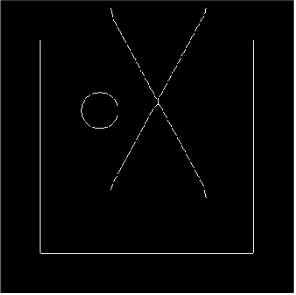
\includegraphics[width=.9\textwidth]{skeletonizeB}
\caption{Skeletonizada}
\end{subfigure}
\caption{Ejemplo de eskeletonize.}\label{fig:3.6}
\end{figure}


\section{Grafos}	
La teoría de grafos~\cite{Wiki:Grafos} en un campo dentro de la computación y de las matemáticas, estudia las propiedades de los grafos son utilizados para representar relaciones habitualmente, y están formados por:
\begin{itemize}
	\item Vértices o nodos: Que representan un objeto, persona o animal del entorno.
	\item Aristas o arcos: Que representan una relación o propiedad que comparten dos nodos, comunicándolos entre si.
Un ejemplo de dos nodos que forman un grafo estará mostrado a continuación en la figura~\ref{fig:3.7}.
\end{itemize}

Es una rama muy amplia pero solo vamos a centrarnos en uno de los problemas que podemos resolver gracias a estas teorías.
\begin{figure}[h]
\centering
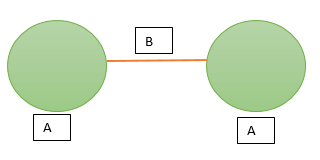
\includegraphics[width=.6\textwidth]{Grafo_Aris_y_Ver}
\caption{A): Son los vértices y B): Es una arista}
\label{fig:3.7}
\end{figure}

\subsection{K-componentes}
Es una de las propiedades del grafo con sus componentes, nos indica cómo de fuertemente conexos están sus nodos o vértices.
Gracias a esta teoría, aprovechamos para afirmar, que un grafo esta dividido en clusters que son, agrupaciones fuertemente conexas de una porción de sus vértices.
Por el problema de los k-componentes, podemos saber qué conjuntos de vértices forman los clusters, aplicado a nuestro problema.
Los vértices que tengan aristas que los comuniquen, pertenecerán a las mismas rectas y de cada conjunto de vértices, sacaremos una recta.

\section{Bordes}
En lo que nos estamos basando para poder resolver el problema,
es en la detección de bordes mediante kernels conocidos.
Para poder detectar donde está el cambio de color en el histograma, y esos cambios bruscos de pigmentación son los que nos indican que eso es un borde.
Para ello se han desarrollado numerosos métodos matemáticos, que pasando una máscara por toda la imagen, nos devuelven otra imagen con los bordes llamada máscara.

En los anexos se encuentra detallado cada uno de ellos, por lo que en adelante sólo nos limitaremos a listarlos.

Kernel \cite{wiki:kernels} \footnote{Dos párrafos mas arriba se usa un Kernel para las operaciones.} Un kernel es una matriz que se operará con una porción de pixeles para suavizar o detectar algún elemento que sea de nuestro interés.

Laplace~\cite{wiki:Laplace}, Prewitt~\cite{wiki:Prewitt}, Scharr~\cite{jon:Scharr}, Sobel~\cite{wiki:Sobel}, Roberts~\cite{wiki:Roberts}, Kirsch~\cite{wiki:Kirsch}, Gabor~\cite{wiki:Gabor}.
 
Aparte de los métodos antes mencionados hemos combinado distintos formas para detectar bordes através de los autovectores \cite{wiki:Eigenvector} largos, de la matriz Hessiana \cite{wiki:Hessiana}.